\documentclass[a4paper,12pt]{article}
\usepackage[top = 2.5cm, bottom = 2.5cm, left = 2.5cm, right = 2.5cm]{geometry}
\usepackage[T1]{fontenc}
\usepackage[utf8]{inputenc}
\usepackage{multirow} 
\usepackage{booktabs} 
\usepackage{graphicx}
\usepackage[spanish]{babel}
\usepackage{setspace}
\setlength{\parindent}{0in}
\usepackage{float}
\usepackage{fancyhdr}
\usepackage{amsmath}
\usepackage{amssymb}
\usepackage{amsthm}
\usepackage[numbers]{natbib}
\newcommand\Mycite[1]{%
	\citeauthor{#1}~[\citeyear{#1}]}
\usepackage{graphicx}
\usepackage{subcaption}
\usepackage{booktabs}
\usepackage{etoolbox}
\usepackage{minibox}
\usepackage{hyperref}
\usepackage{xcolor}
\usepackage[skins]{tcolorbox}
%---------------------------

\newtcolorbox{cajita}[1][]{
	 #1
}

\newenvironment{sol}
{\renewcommand\qedsymbol{$\square$}\begin{proof}[\textbf{Solución.}]}
	{\end{proof}}

\newenvironment{dem}
{\renewcommand\qedsymbol{$\blacksquare$}\begin{proof}[\textbf{Demostración.}]}
	{\end{proof}}

\newtheorem{problema}{Problema}
\newtheorem{definicion}{Definición}
\newtheorem{ejemplo}{Ejemplo}
\newtheorem{teorema}{Teorema}
\newtheorem{corolario}{Corolario}[teorema]
\newtheorem{lema}[teorema]{Lema}
\newtheorem{prop}{Proposición}
\newtheorem*{nota}{\textbf{NOTA}}
\renewcommand\qedsymbol{$\blacksquare$}
\usepackage{svg}
\usepackage{tikz}
\usepackage[framemethod=default]{mdframed}
\global\mdfdefinestyle{exampledefault}{%
linecolor=lightgray,linewidth=1pt,%
leftmargin=1cm,rightmargin=1cm,
}




\newenvironment{noter}[1]{%
\mdfsetup{%
frametitle={\tikz\node[fill=white,rectangle,inner sep=0pt,outer sep=0pt]{#1};},
frametitleaboveskip=-0.5\ht\strutbox,
frametitlealignment=\raggedright
}%
\begin{mdframed}[style=exampledefault]
}{\end{mdframed}}
\newcommand{\linea}{\noindent\rule{\textwidth}{3pt}}
\newcommand{\linita}{\noindent\rule{\textwidth}{1pt}}

\AtBeginEnvironment{align}{\setcounter{equation}{0}}
\pagestyle{fancy}

\fancyhf{}









%----------------------------------------------------------
\lhead{\footnotesize Data Mining}
\rhead{\footnotesize  Armas, Billingslea, Rompich}
\cfoot{\footnotesize \thepage}


%--------------------------

\begin{document}
 \thispagestyle{empty} 
    \begin{tabular}{p{15.5cm}}
    \begin{tabbing}
    \textbf{Universidad del Valle de Guatemala} \\
    Ejercicio en clase - Grupo 5 \\\\

   \textbf{Estudiante:} Esteban Armas, Jackelin Billingslea, Rudik Rompich\\
   \textbf{Correos:} \href{mailto:arm19371@uvg.edu.gt}{arm19371@uvg.edu.gt},\href{mailto:bil19161@uvg.edu.gt}{bil19161@uvg.edu.gt}, \href{mailto:rom19857@uvg.edu.gt}{rom19857@uvg.edu.gt}\\
   \textbf{Carnés:} 19371, 19161, 19857
    \end{tabbing}
    \begin{center}
        IA3028 - Data Mining - Catedrático: Luis Pedro Flores\\
        \today
    \end{center}\\
    \hline
    \\
    \end{tabular} 
    \vspace*{0.3cm} 
    \begin{center} 
    {\Large \bf  PowerBI + Estadística Descriptiva
} 
        \vspace{2mm}
    \end{center}
    \vspace{0.4cm}
%--------------------------

\begin{enumerate}
	\item ¿Qué restaurante vende más? Colocar el valor en monto (\$).
	\begin{sol}
		Según la métrica propuesta (sumatoria del precio del producto por la cantidad), como se observa en \ref{fig: 1}, el restaurante que tiene más ventas es el segundo con \$683,865.90 en ventas; en comparación al primer restaurante, que tiene ventas de \$490,489.42.
			\begin{figure}[H]
			\centering
			$\begin{array}{cc}
				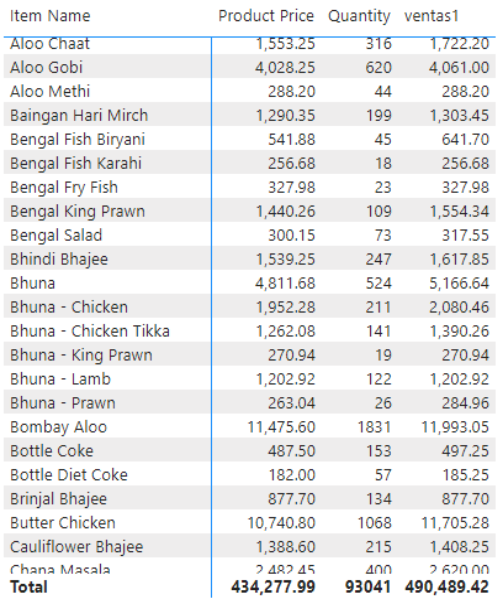
\includegraphics[scale=0.4]{Images/1}& 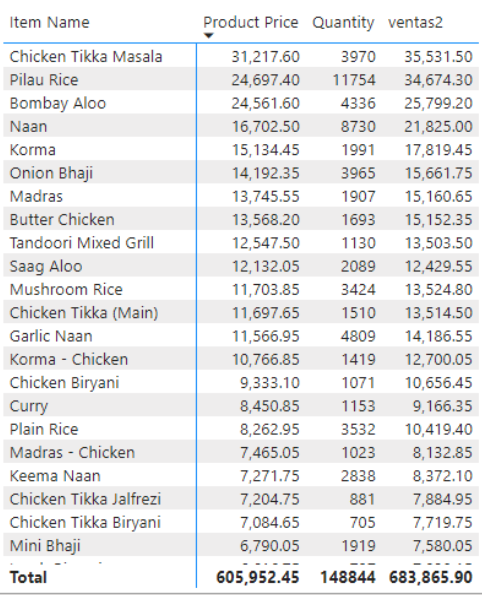
\includegraphics[scale=0.4]{Images/1.1}\\
				\text{Restaurante 1} & \text{Restaurante 2}
			\end{array}$
			\caption{Ventas}
			\label{fig: 1}
		\end{figure}

	\end{sol}
	\item ¿Qué unidades de venta tiene cada producto?
		\begin{sol}
			Para visualizar las unidades de venta de cada producto se seleccionaron los 20 productos con mayores unidades de venta y se optó por gráficos de barras (véase \ref{fig: 2}, \ref{fig: 3}) , para una mejor percepción de los datos. Nótese que los primeros dos productos son iguales en ambos restaurantes. 
		\begin{figure}[H]
			\centering
			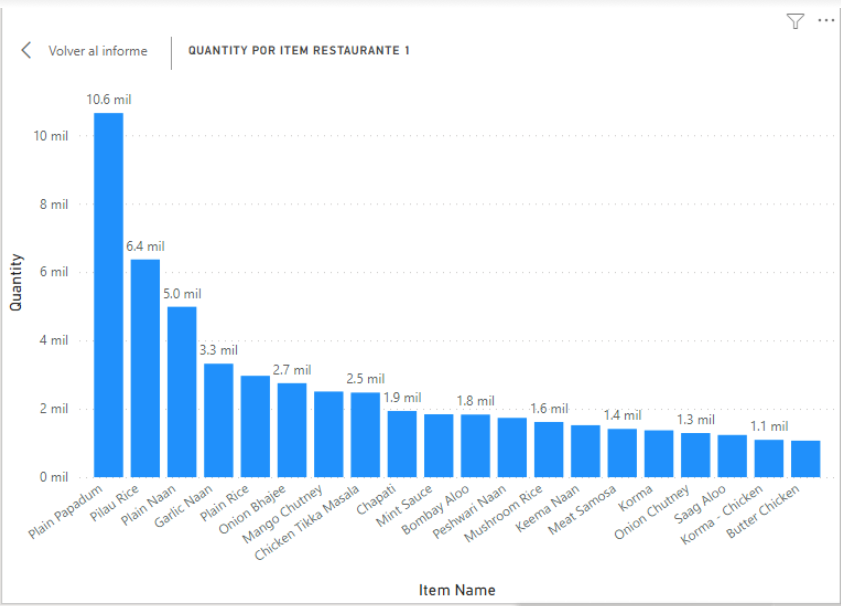
\includegraphics[scale=0.3]{Images/2}
			\caption{Unidades de venta del restaurante 1}
			\label{fig: 2}
		\end{figure}
	\begin{figure}[H]
		\centering
		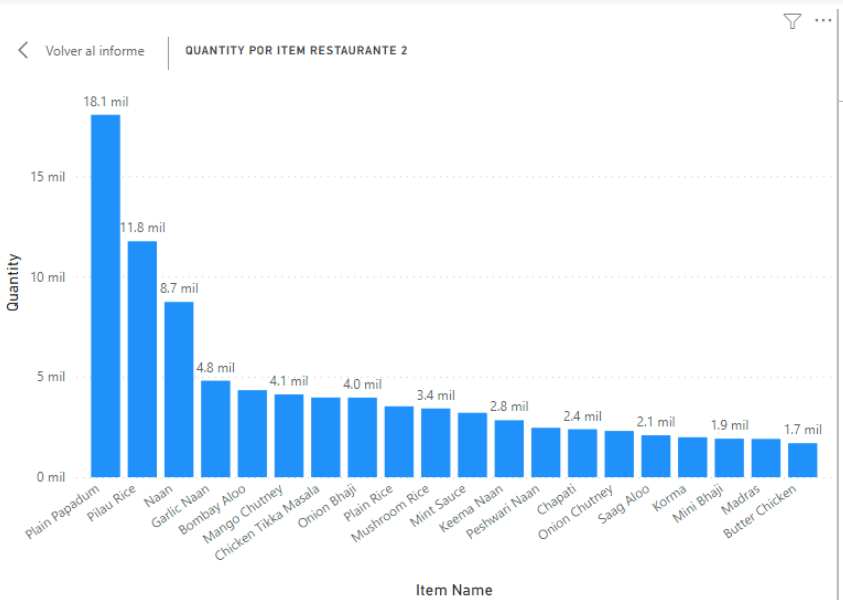
\includegraphics[scale=0.3]{Images/2.1}
		\caption{Unidades de venta del restaurante 2}
		\label{fig: 3}
	\end{figure}
	\end{sol}
	\item Haga un análisis de los precios de los productos. (Utilice las medidas de tendencia central y desviación para contestar esta pregunta) Utilice promedio, desviación, valores máximos y mínimos y el valor de la mediana para esto.
		\begin{sol}
		Los resultados del restaurante 1 (véase \ref{fig: 4}) y del restaurante 2 (véase \ref{fig: 5}) muestran lo siguiente: 
		\begin{enumerate}
			\item La mayor parte de la dispersión de los precios de los productos del primer restaurante se encuentran en 8.79$\pm$3.67, mientras que los del segundo restaurante en 8.08$\pm$3.07.
			\item Nótese que en ambos restaurantes la mediana es mayor a la media; esto significa que los datos se encuentran sesgados hacia la izquierda moderadamente (ya que las medianas no sobrepasan por 1 punto a la media). Una interpretación directa sería que existen varios productos que tienen precios de los productos cercanos a la media; pero muchos que sobrepasan la media y pocos que son menores a la media. 
			\item Los máximos y mínimos no tienen una utilidad evidente con la data proporcionada; simplemente representan datos atípicos que no afectan al conjunto en general. 
		\end{enumerate}
\begin{figure}[H]
	\centering
	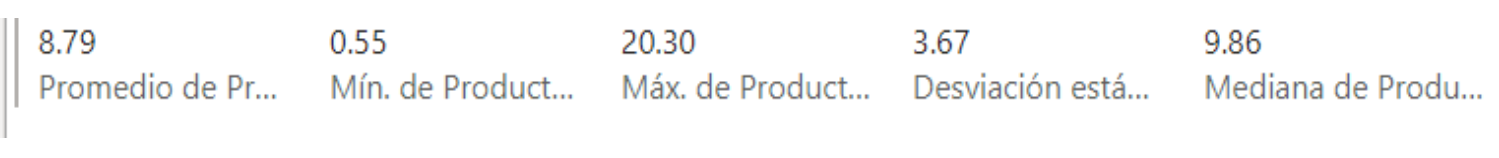
\includegraphics[scale=0.2]{Images/3}
	\caption{Análisis del restaurante 1}
	\label{fig: 4}
\end{figure}
\begin{figure}[H]
	\centering
	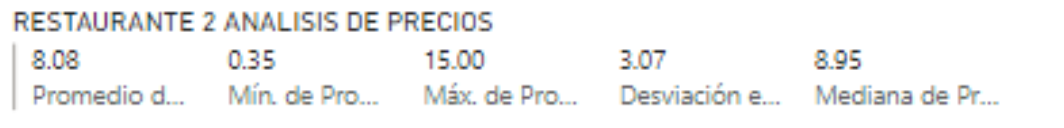
\includegraphics[scale=0.3]{Images/3.1}
	\caption{Análisis del restaurante 2}
	\label{fig: 5}
\end{figure}
	\end{sol}
	\item ¿Cuál es el promedio mensual de venta durante el 2019?
		\begin{sol}
		Los datos obtenidos se encuentran en \ref{fig: 6} y \ref{fig: 7}. El requerimiento es encontrar la media (promedio) de los restaurantes durante 2019. Nótese que el promedio del restaurante 1 es \$ 14,513.65 y del restaurante 2 es \$6,675.571. Sin embargo, en el mes de agosto las ventas se desplomaron (por alguna causa atípica, no determinada) por lo cual los datos evidentemente están sesgados y la media no podría ser una variante determinante al momento de un análisis más profundo.  
\begin{figure}[H]
	\centering
	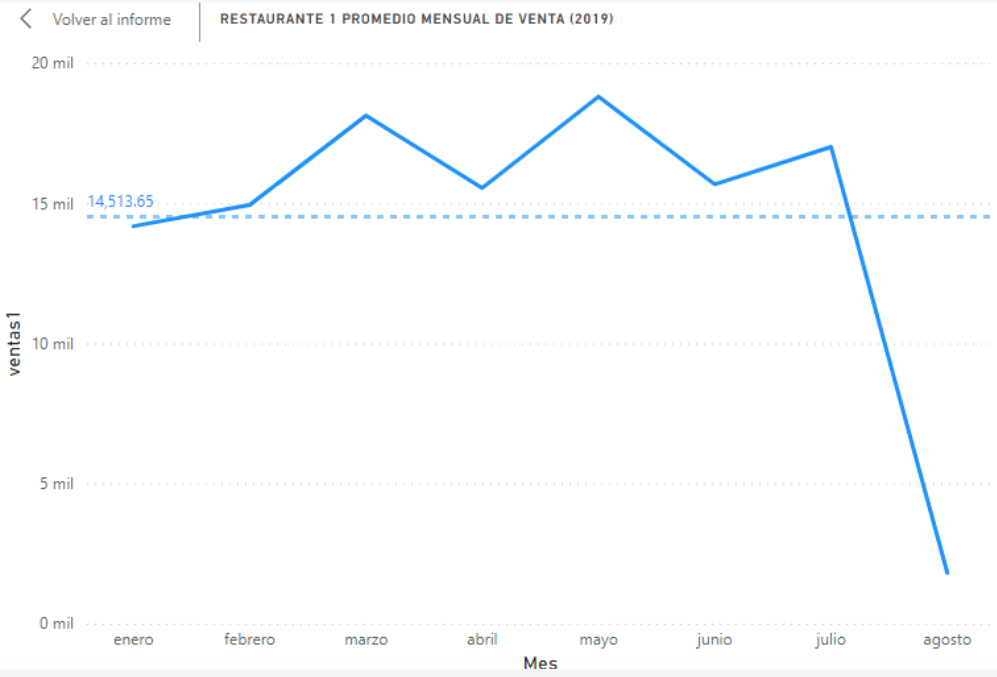
\includegraphics[scale=0.3]{Images/4}
	\caption{Unidades de venta del restaurante 1}
	\label{fig: 6}
\end{figure}
\begin{figure}[H]
	\centering
	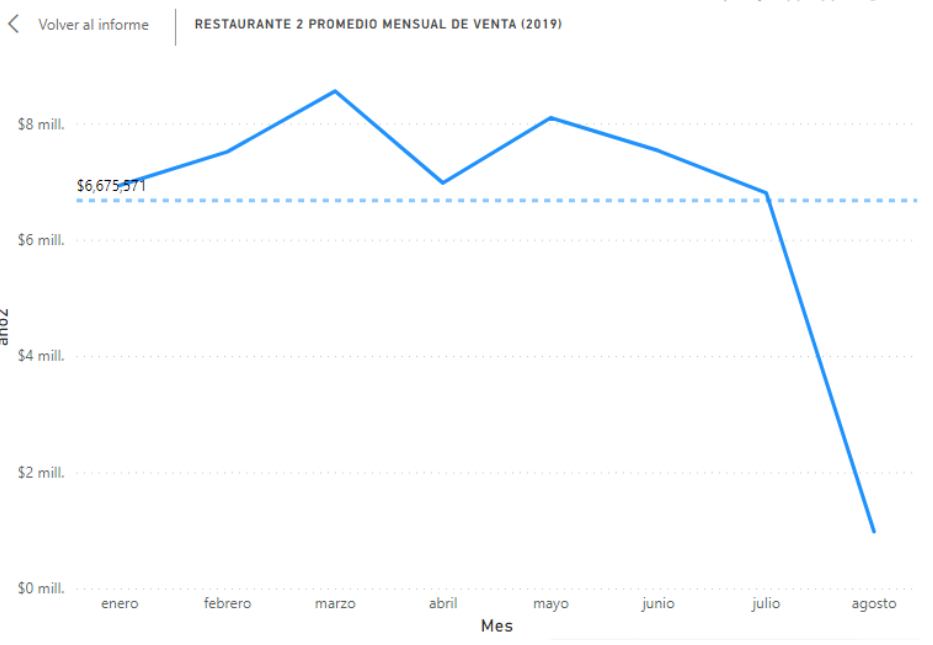
\includegraphics[scale=0.3]{Images/4.1}
	\caption{Unidades de venta del restaurante 2}
	\label{fig: 7}
\end{figure}
	\end{sol}
	
	\item Elabore un tablero de información con la diferencia de ambas.
	
		\begin{sol}
		El tablero de Power BI consiste en los incisos anteriormente descritos.
		\begin{center}
			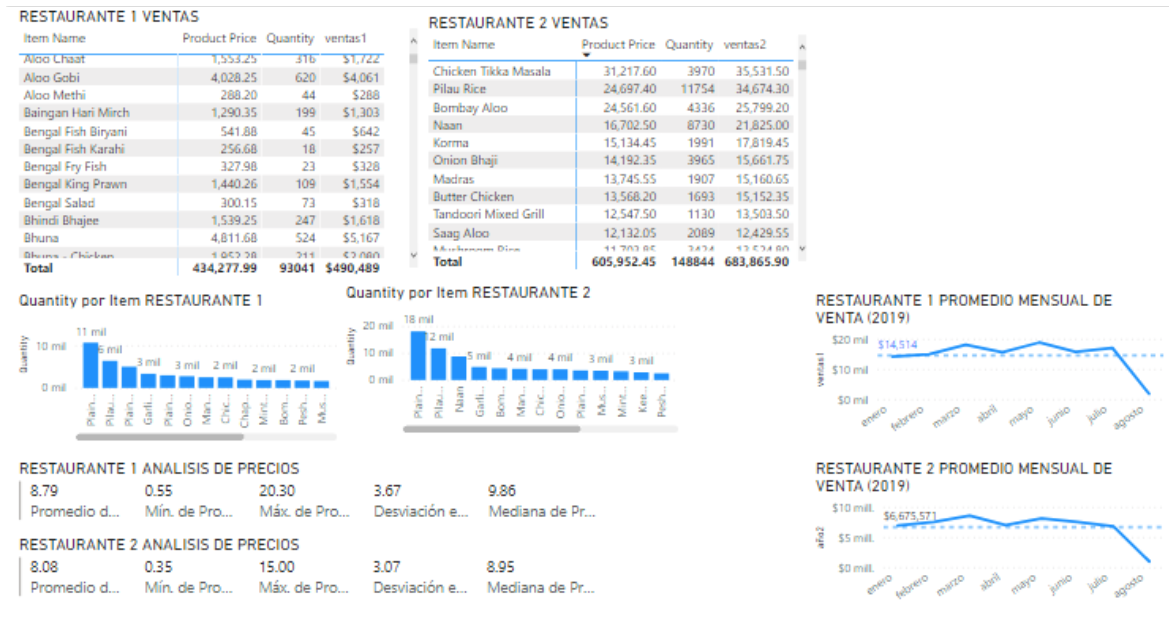
\includegraphics[scale=0.35]{Images/5}
		\end{center}
	\end{sol}
\end{enumerate}


%---------------------------
%\bibliographystyle{apa}
%\bibliography{referencias.bib}

\end{document}